\documentclass[a4paper]{scrartcl}\usepackage[]{graphicx}\usepackage[]{color}
% maxwidth is the original width if it is less than linewidth
% otherwise use linewidth (to make sure the graphics do not exceed the margin)
\makeatletter
\def\maxwidth{ %
  \ifdim\Gin@nat@width>\linewidth
    \linewidth
  \else
    \Gin@nat@width
  \fi
}
\makeatother

\definecolor{fgcolor}{rgb}{0.345, 0.345, 0.345}
\newcommand{\hlnum}[1]{\textcolor[rgb]{0.686,0.059,0.569}{#1}}%
\newcommand{\hlstr}[1]{\textcolor[rgb]{0.192,0.494,0.8}{#1}}%
\newcommand{\hlcom}[1]{\textcolor[rgb]{0.678,0.584,0.686}{\textit{#1}}}%
\newcommand{\hlopt}[1]{\textcolor[rgb]{0,0,0}{#1}}%
\newcommand{\hlstd}[1]{\textcolor[rgb]{0.345,0.345,0.345}{#1}}%
\newcommand{\hlkwa}[1]{\textcolor[rgb]{0.161,0.373,0.58}{\textbf{#1}}}%
\newcommand{\hlkwb}[1]{\textcolor[rgb]{0.69,0.353,0.396}{#1}}%
\newcommand{\hlkwc}[1]{\textcolor[rgb]{0.333,0.667,0.333}{#1}}%
\newcommand{\hlkwd}[1]{\textcolor[rgb]{0.737,0.353,0.396}{\textbf{#1}}}%
\let\hlipl\hlkwb

\usepackage{framed}
\makeatletter
\newenvironment{kframe}{%
 \def\at@end@of@kframe{}%
 \ifinner\ifhmode%
  \def\at@end@of@kframe{\end{minipage}}%
  \begin{minipage}{\columnwidth}%
 \fi\fi%
 \def\FrameCommand##1{\hskip\@totalleftmargin \hskip-\fboxsep
 \colorbox{shadecolor}{##1}\hskip-\fboxsep
     % There is no \\@totalrightmargin, so:
     \hskip-\linewidth \hskip-\@totalleftmargin \hskip\columnwidth}%
 \MakeFramed {\advance\hsize-\width
   \@totalleftmargin\z@ \linewidth\hsize
   \@setminipage}}%
 {\par\unskip\endMakeFramed%
 \at@end@of@kframe}
\makeatother

\definecolor{shadecolor}{rgb}{.97, .97, .97}
\definecolor{messagecolor}{rgb}{0, 0, 0}
\definecolor{warningcolor}{rgb}{1, 0, 1}
\definecolor{errorcolor}{rgb}{1, 0, 0}
\newenvironment{knitrout}{}{} % an empty environment to be redefined in TeX

\usepackage{alltt}
\usepackage{lscape}
\usepackage[section]{placeins}
\usepackage{rotating}
\usepackage[margin=1.0in]{geometry}
\usepackage[table]{xcolor}
\usepackage[hidelinks]{hyperref}
\renewcommand{\textfraction}{0.05}
\renewcommand{\topfraction}{0.8}
\renewcommand{\bottomfraction}{0.8}
\renewcommand{\floatpagefraction}{0.75}
\IfFileExists{upquote.sty}{\usepackage{upquote}}{}
\begin{document}

\title{A Population Genetic Report}


\subtitle {using PopGenReport Version  3.0.4 }

\author{Adamack \& Gruber}
\maketitle

\begin{itemize}
  \item Adamack, A. T., Gruber, B. (2014), PopGenReport: simplifying basic population genetic analyses in R. \emph{Methods in Ecology and Evolution}, 5: 384-387. \href{http://onlinelibrary.wiley.com/doi/10.1111/2041-210X.12158/full}{doi: 10.1111/2041-210X.12158}.
  \item Gruber, B. and Adamack, A. T. (2015), landgenreport: a new r function to simplify landscape genetic analysis using resistance surface layers. \emph{Molecular Ecology Resources}, 15: 1172-1178. \href{http://onlinelibrary.wiley.com/doi/10.1111/1755-0998.12381/full}{doi: 10.1111/1755-0998.12381}.
\end{itemize}


%<<echo=FALSE, results='asis'>>=
%rref <- citation("PopGenReport")
%print(rref[1], style="latex")
%@
  
%<<echo=FALSE, results='asis'>>=
%print(rref[2], style="latex")
%@

\tableofcontents
\newpage


\section{Counts}
This analysis looks at 322 individuals.

\noindent
\newline The mean number of alleles per locus (across all locations): 11.2


\noindent
\newline The percentage of missing data was 0.6\%.

\begin{knitrout}
\definecolor{shadecolor}{rgb}{0.969, 0.969, 0.969}\color{fgcolor}
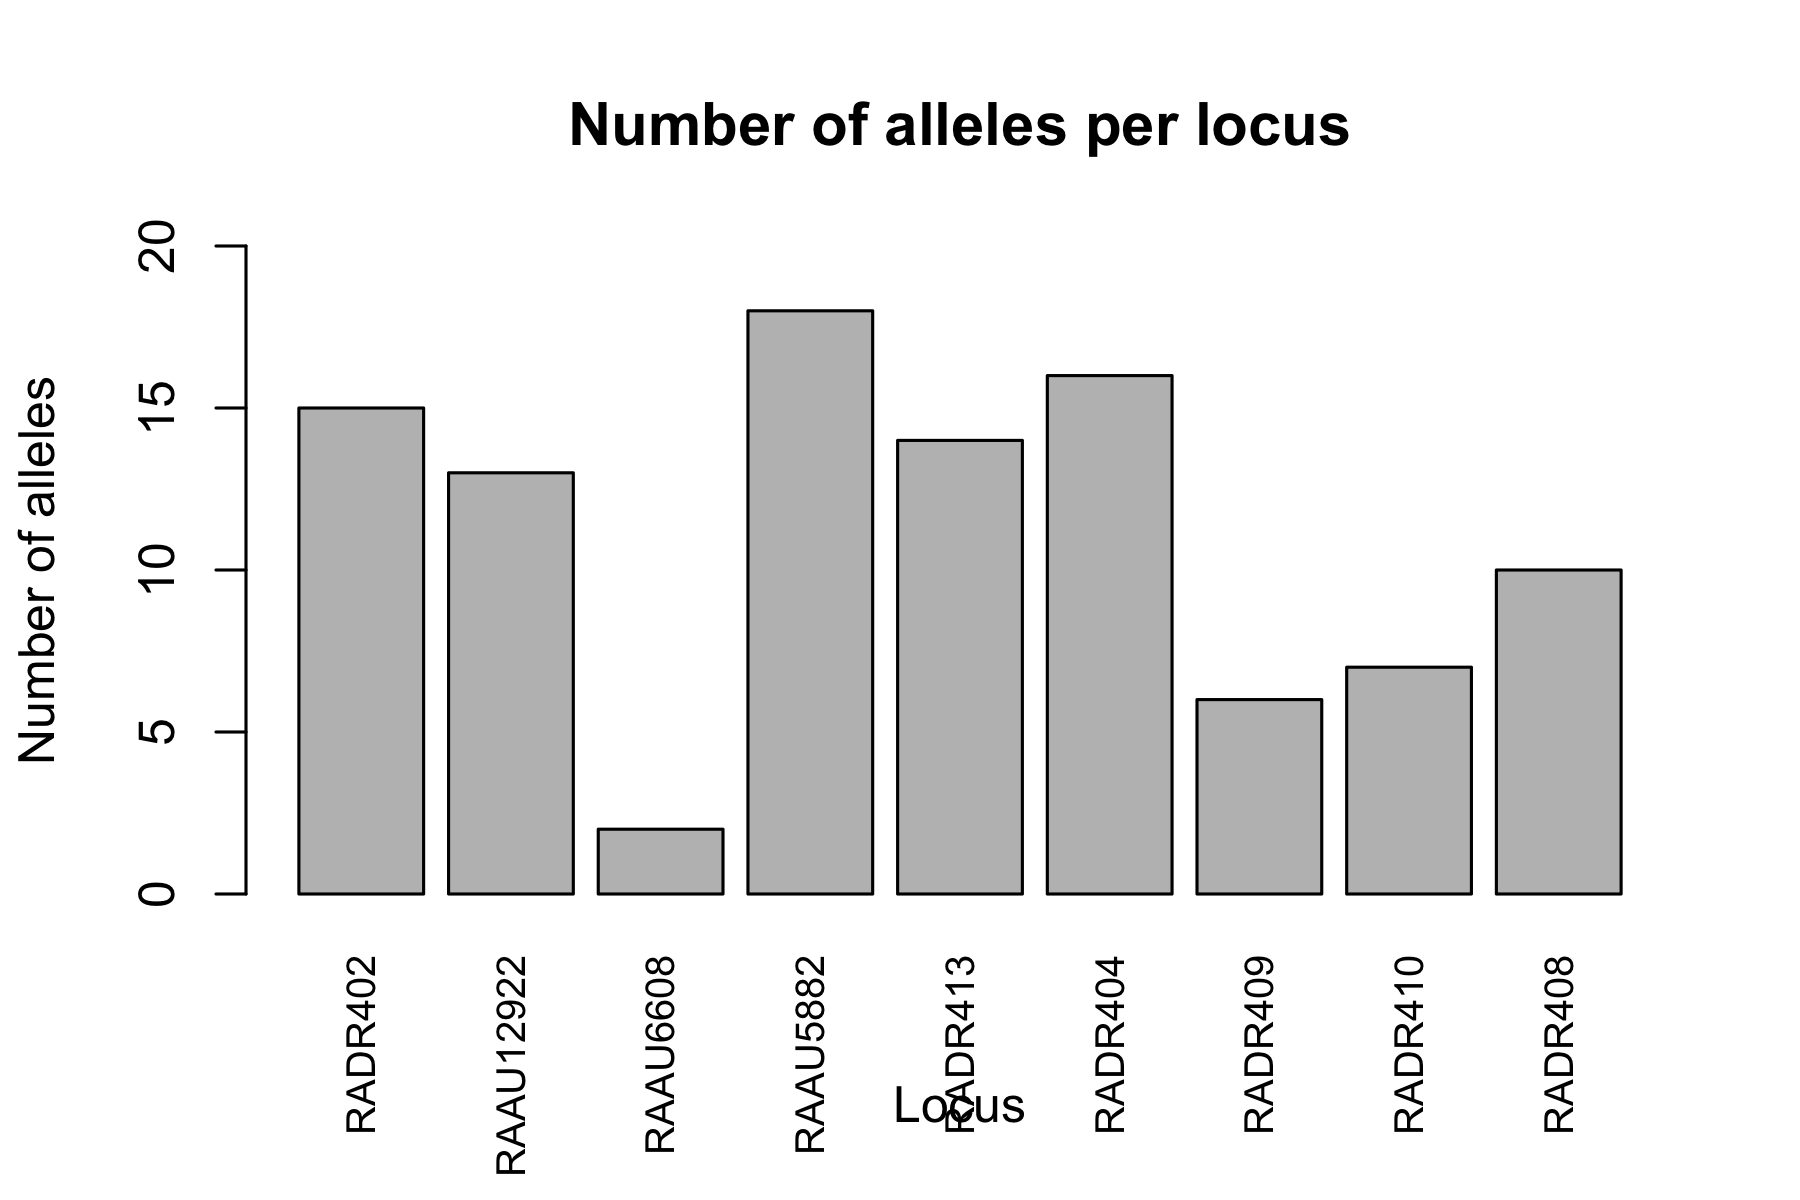
\includegraphics[width=\maxwidth]{PopGenReport-n_alleles_per_locus-1} 
\end{knitrout}
\FloatBarrier



\noindent 
\newline The individuals were sampled from the following locations in the following numbers: 


% latex table generated in R 4.1.1 by xtable 1.8-4 package
% Thu Oct 21 12:17:31 2021
\begin{table}[ht]
\centering
\begin{tabular}{llllllllll}
   \hline
population & Abbey\_RA1231 & Audub\_RA0639 & Beave\_OR0099 & Borde\_RA1443 & Brook\_RA0774 & Butle\_RA0878 & Canem\_OR0311 & Cedar\_RA1270 & Chris\_OR0244 \\ 
   \rowcolor[gray]{0.9} \# ind & 16 & 18 & 32 & 12 & 18 & 16 & 20 & 17 & 7 \\ 
  population & CoopM\_OR0291 & Foste\_RA0793 & Gabbe\_RA0808 & Hylan\_RA1790 & LPowe\_RA0670 & OaksB\_RA0721 & Powel\_RA0759 & Tadpo\_RA1832 & Timbe\_OR0163 \\ 
   \rowcolor[gray]{0.9} \# ind & 28 & 5 & 8 & 20 & 18 & 16 & 17 & 19 & 5 \\ 
  population & Unit2\_OR0328 & Veter\_RA0800 & Water\_RA0616 &  &  &  &  &  &  \\ 
   \rowcolor[gray]{0.9} \# ind & 7 & 18 & 5 &  &  &  &  &  &  \\ 
   \hline
\end{tabular}
\caption{Number of individuals per population} 
\end{table}


\noindent
\newline {The total number of alleles sampled across all locations was {101}} 
\newline The total number of alleles seen in each sampling location was:



% latex table generated in R 4.1.1 by xtable 1.8-4 package
% Thu Oct 21 12:17:31 2021
\begin{table}[ht]
\centering
\begin{tabular}{llllllllll}
   \hline
population & Abbey\_RA1231 & Audub\_RA0639 & Beave\_OR0099 & Borde\_RA1443 & Brook\_RA0774 & Butle\_RA0878 & Canem\_OR0311 & Cedar\_RA1270 & Chris\_OR0244 \\ 
   \rowcolor[gray]{0.9} \# alleles & 53 & 44 & 69 & 52 & 59 & 58 & 61 & 53 & 40 \\ 
  population & CoopM\_OR0291 & Foste\_RA0793 & Gabbe\_RA0808 & Hylan\_RA1790 & LPowe\_RA0670 & OaksB\_RA0721 & Powel\_RA0759 & Tadpo\_RA1832 & Timbe\_OR0163 \\ 
   \rowcolor[gray]{0.9} \# alleles & 55 & 39 & 40 & 32 & 57 & 63 & 51 & 46 & 37 \\ 
  population & Unit2\_OR0328 & Veter\_RA0800 & Water\_RA0616 &  &  &  &  &  &  \\ 
   \rowcolor[gray]{0.9} \# alleles & 38 & 51 & 42 &  &  &  &  &  &  \\ 
   \hline
\end{tabular}
\caption{Number of alleles per population} 
\end{table}

\begin{knitrout}
\definecolor{shadecolor}{rgb}{0.969, 0.969, 0.969}\color{fgcolor}
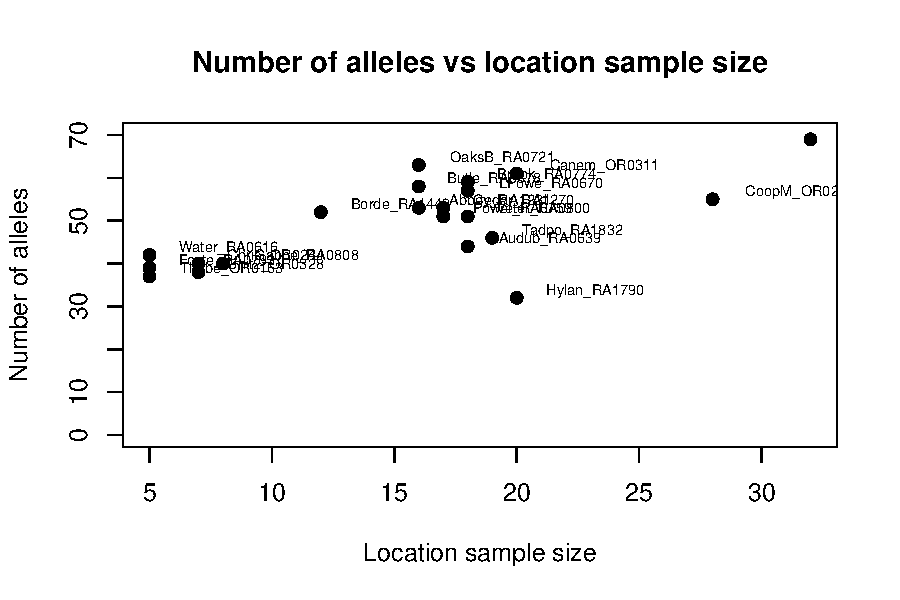
\includegraphics[width=\maxwidth]{PopGenReport-pop_sampsz_vs_alleles-1} 
\end{knitrout}
\FloatBarrier
\noindent
\newline The number of alleles per locus (across all subpopulations):


% latex table generated in R 4.1.1 by xtable 1.8-4 package
% Thu Oct 21 12:17:31 2021
\begin{table}[ht]
\centering
\begin{tabular}{llllllll}
   \hline
locus & RADR402 & RAAU12922 & RAAU6608 & RAAU5882 & RADR413 & RADR404 & RADR409 \\ 
   \rowcolor[gray]{0.9} \# alleles & 15 & 13 & 2 & 18 & 14 & 16 & 6 \\ 
  locus & RADR410 & RADR408 &  &  &  &  &  \\ 
   \rowcolor[gray]{0.9} \# alleles & 7 & 10 &  &  &  &  &  \\ 
   \hline
\end{tabular}
\caption{Number of alleles per locus across all subpopulations} 
\end{table}







\FloatBarrier


\section{Hs and Ht based population differentiation statistics}



% latex table generated in R 4.1.1 by xtable 1.8-4 package
% Thu Oct 21 12:17:31 2021
\begin{table}[ht]
\centering
\begin{tabular}{rrrrrr}
  \hline
 & Hs & Ht & Gst & Gprime\_st & D \\ 
  \hline
RADR402 & 0.825 & 0.872 & 0.054 & 0.323 & 0.282 \\ 
   \rowcolor[gray]{0.9} RAAU12922 & 0.813 & 0.861 & 0.056 & 0.311 & 0.268 \\ 
  RAAU6608 & 0.038 & 0.041 & 0.066 & 0.072 & 0.003 \\ 
   \rowcolor[gray]{0.9} RAAU5882 & 0.734 & 0.796 & 0.079 & 0.309 & 0.247 \\ 
  RADR413 & 0.831 & 0.856 & 0.028 & 0.176 & 0.151 \\ 
   \rowcolor[gray]{0.9} RADR404 & 0.817 & 0.881 & 0.073 & 0.417 & 0.369 \\ 
  RADR409 & 0.590 & 0.656 & 0.101 & 0.258 & 0.170 \\ 
   \rowcolor[gray]{0.9} RADR410 & 0.555 & 0.580 & 0.042 & 0.100 & 0.058 \\ 
  RADR408 & 0.791 & 0.849 & 0.069 & 0.344 & 0.293 \\ 
   \rowcolor[gray]{0.9}  \hline
\end{tabular}
\caption{Hs and Ht based estimates of differentiation: Gst, Gst and Dest for each locus} 
\end{table}
% latex table generated in R 4.1.1 by xtable 1.8-4 package
% Thu Oct 21 12:17:31 2021
\begin{table}[ht]
\centering
\begin{tabular}{rrrrrr}
  \hline
Hs & Ht & Gst\_est & Gprime\_st & D\_het & D\_mean \\ 
  \hline
0.666 & 0.710 & 0.062 & 0.195 & 0.139 & 0.023 \\ 
   \rowcolor[gray]{0.9}  \hline
\end{tabular}
\caption{Hs and Ht based global estimates of differentiation: Gst, Gst and Dest for each locus} 
\end{table}





% latex table generated in R 4.1.1 by xtable 1.8-4 package
% Thu Oct 21 12:17:51 2021
\begin{sidewaystable}[ht]
\centering
\scalebox{0.88}{
\begin{tabular}{rrrrrrrrrrrrrrrrrrrrrr}
  \hline
 & Abbey\_RA1231 & Audub\_RA0639 & Beave\_OR0099 & Borde\_RA1443 & Brook\_RA0774 & Butle\_RA0878 & Canem\_OR0311 & Cedar\_RA1270 & Chris\_OR0244 & CoopM\_OR0291 & Foste\_RA0793 & Gabbe\_RA0808 & Hylan\_RA1790 & LPowe\_RA0670 & OaksB\_RA0721 & Powel\_RA0759 & Tadpo\_RA1832 & Timbe\_OR0163 & Unit2\_OR0328 & Veter\_RA0800 & Water\_RA0616 \\ 
  \hline
Abbey\_RA1231 &  &  &  &  &  &  &  &  &  &  &  &  &  &  &  &  &  &  &  &  &  \\ 
  Audub\_RA0639 & 0.084 &  &  &  &  &  &  &  &  &  &  &  &  &  &  &  &  &  &  &  &  \\ 
  Beave\_OR0099 & 0.035 & 0.091 &  &  &  &  &  &  &  &  &  &  &  &  &  &  &  &  &  &  &  \\ 
  Borde\_RA1443 & 0.123 & 0.129 & 0.155 &  &  &  &  &  &  &  &  &  &  &  &  &  &  &  &  &  &  \\ 
  Brook\_RA0774 & 0.102 & 0.115 & 0.078 & 0.050 &  &  &  &  &  &  &  &  &  &  &  &  &  &  &  &  &  \\ 
  Butle\_RA0878 & 0.067 & 0.073 & 0.094 & 0.071 & 0.082 &  &  &  &  &  &  &  &  &  &  &  &  &  &  &  &  \\ 
  Canem\_OR0311 & 0.058 & 0.103 & 0.086 & 0.106 & 0.066 & 0.019 &  &  &  &  &  &  &  &  &  &  &  &  &  &  &  \\ 
  Cedar\_RA1270 & 0.072 & 0.078 & 0.086 & 0.124 & 0.060 & 0.079 & 0.101 &  &  &  &  &  &  &  &  &  &  &  &  &  &  \\ 
  Chris\_OR0244 & 0.160 & 0.217 & 0.115 & 0.264 & 0.269 & 0.199 & 0.186 & 0.220 &  &  &  &  &  &  &  &  &  &  &  &  &  \\ 
  CoopM\_OR0291 & 0.163 & 0.215 & 0.135 & 0.192 & 0.140 & 0.113 & 0.136 & 0.187 & 0.284 &  &  &  &  &  &  &  &  &  &  &  &  \\ 
  Foste\_RA0793 & 0.093 & 0.152 & 0.090 & 0.109 & 0.003 & 0.116 & 0.108 & 0.052 & 0.347 & 0.127 &  &  &  &  &  &  &  &  &  &  &  \\ 
  Gabbe\_RA0808 & 0.180 & 0.246 & 0.186 & 0.229 & 0.114 & 0.183 & 0.146 & 0.128 & 0.367 & 0.176 & 0.123 &  &  &  &  &  &  &  &  &  &  \\ 
  Hylan\_RA1790 & 0.219 & 0.303 & 0.214 & 0.267 & 0.225 & 0.283 & 0.242 & 0.265 & 0.328 & 0.337 & 0.272 & 0.253 &  &  &  &  &  &  &  &  &  \\ 
  LPowe\_RA0670 & 0.078 & 0.111 & 0.077 & 0.062 & 0.039 & 0.079 & 0.084 & 0.079 & 0.206 & 0.113 & 0.063 & 0.141 & 0.184 &  &  &  &  &  &  &  &  \\ 
  OaksB\_RA0721 & 0.055 & 0.101 & 0.091 & 0.114 & 0.062 & 0.024 & 0.037 & 0.039 & 0.246 & 0.142 & 0.082 & 0.041 & 0.176 & 0.045 &  &  &  &  &  &  &  \\ 
  Powel\_RA0759 & 0.056 & 0.152 & 0.091 & 0.083 & 0.053 & 0.076 & 0.064 & 0.108 & 0.201 & 0.159 & 0.161 & 0.191 & 0.195 & 0.053 & 0.069 &  &  &  &  &  &  \\ 
  Tadpo\_RA1832 & 0.096 & 0.128 & 0.072 & 0.203 & 0.193 & 0.161 & 0.164 & 0.155 & 0.123 & 0.214 & 0.211 & 0.214 & 0.233 & 0.125 & 0.164 & 0.160 &  &  &  &  &  \\ 
  Timbe\_OR0163 & 0.093 & 0.111 & 0.008 & 0.149 & 0.066 & 0.066 & 0.064 & 0.073 & 0.052 & 0.137 & 0.155 & 0.179 & 0.247 & 0.105 & 0.110 & 0.103 & 0.081 &  &  &  &  \\ 
  Unit2\_OR0328 & 0.089 & 0.163 & 0.031 & 0.148 & 0.096 & 0.091 & 0.106 & 0.155 & 0.093 & 0.134 & 0.106 & 0.253 & 0.243 & 0.081 & 0.138 & 0.145 & 0.153 & -0.024 &  &  &  \\ 
  Veter\_RA0800 & 0.142 & 0.154 & 0.122 & 0.226 & 0.119 & 0.157 & 0.182 & 0.125 & 0.308 & 0.214 & 0.079 & 0.141 & 0.260 & 0.122 & 0.124 & 0.206 & 0.151 & 0.146 & 0.140 &  &  \\ 
  Water\_RA0616 & 0.103 & 0.118 & 0.120 & -0.012 & 0.077 & -0.049 & 0.032 & 0.120 & 0.213 & 0.120 & 0.148 & 0.235 & 0.308 & 0.084 & 0.058 & 0.051 & 0.143 & 0.086 & 0.110 & 0.227 &  \\ 
   \hline
\end{tabular}
}
\caption{mmod Jost's D pairwise} 
\end{sidewaystable}
% latex table generated in R 4.1.1 by xtable 1.8-4 package
% Thu Oct 21 12:17:51 2021
\begin{sidewaystable}[ht]
\centering
\scalebox{0.88}{
\begin{tabular}{rrrrrrrrrrrrrrrrrrrrrr}
  \hline
 & Abbey\_RA1231 & Audub\_RA0639 & Beave\_OR0099 & Borde\_RA1443 & Brook\_RA0774 & Butle\_RA0878 & Canem\_OR0311 & Cedar\_RA1270 & Chris\_OR0244 & CoopM\_OR0291 & Foste\_RA0793 & Gabbe\_RA0808 & Hylan\_RA1790 & LPowe\_RA0670 & OaksB\_RA0721 & Powel\_RA0759 & Tadpo\_RA1832 & Timbe\_OR0163 & Unit2\_OR0328 & Veter\_RA0800 & Water\_RA0616 \\ 
  \hline
Abbey\_RA1231 &  &  &  &  &  &  &  &  &  &  &  &  &  &  &  &  &  &  &  &  &  \\ 
  Audub\_RA0639 & 0.122 &  &  &  &  &  &  &  &  &  &  &  &  &  &  &  &  &  &  &  &  \\ 
  Beave\_OR0099 & 0.050 & 0.130 &  &  &  &  &  &  &  &  &  &  &  &  &  &  &  &  &  &  &  \\ 
  Borde\_RA1443 & 0.170 & 0.186 & 0.210 &  &  &  &  &  &  &  &  &  &  &  &  &  &  &  &  &  &  \\ 
  Brook\_RA0774 & 0.144 & 0.169 & 0.110 & 0.073 &  &  &  &  &  &  &  &  &  &  &  &  &  &  &  &  &  \\ 
  Butle\_RA0878 & 0.092 & 0.105 & 0.128 & 0.099 & 0.115 &  &  &  &  &  &  &  &  &  &  &  &  &  &  &  &  \\ 
  Canem\_OR0311 & 0.082 & 0.149 & 0.118 & 0.147 & 0.094 & 0.027 &  &  &  &  &  &  &  &  &  &  &  &  &  &  &  \\ 
  Cedar\_RA1270 & 0.103 & 0.115 & 0.120 & 0.173 & 0.088 & 0.111 & 0.142 &  &  &  &  &  &  &  &  &  &  &  &  &  &  \\ 
  Chris\_OR0244 & 0.222 & 0.303 & 0.161 & 0.352 & 0.361 & 0.267 & 0.253 & 0.300 &  &  &  &  &  &  &  &  &  &  &  &  &  \\ 
  CoopM\_OR0291 & 0.220 & 0.293 & 0.182 & 0.258 & 0.195 & 0.154 & 0.186 & 0.253 & 0.373 &  &  &  &  &  &  &  &  &  &  &  &  \\ 
  Foste\_RA0793 & 0.130 & 0.215 & 0.124 & 0.152 & 0.004 & 0.158 & 0.150 & 0.075 & 0.444 & 0.175 &  &  &  &  &  &  &  &  &  &  &  \\ 
  Gabbe\_RA0808 & 0.250 & 0.342 & 0.253 & 0.312 & 0.167 & 0.250 & 0.204 & 0.185 & 0.476 & 0.244 & 0.176 &  &  &  &  &  &  &  &  &  &  \\ 
  Hylan\_RA1790 & 0.313 & 0.428 & 0.303 & 0.375 & 0.326 & 0.387 & 0.341 & 0.374 & 0.452 & 0.453 & 0.380 & 0.367 &  &  &  &  &  &  &  &  &  \\ 
  LPowe\_RA0670 & 0.111 & 0.161 & 0.108 & 0.090 & 0.058 & 0.111 & 0.119 & 0.114 & 0.283 & 0.158 & 0.091 & 0.202 & 0.272 &  &  &  &  &  &  &  &  \\ 
  OaksB\_RA0721 & 0.078 & 0.145 & 0.125 & 0.158 & 0.089 & 0.034 & 0.052 & 0.056 & 0.327 & 0.193 & 0.115 & 0.060 & 0.257 & 0.065 &  &  &  &  &  &  &  \\ 
  Powel\_RA0759 & 0.082 & 0.218 & 0.128 & 0.119 & 0.078 & 0.108 & 0.092 & 0.156 & 0.279 & 0.219 & 0.223 & 0.268 & 0.289 & 0.078 & 0.100 &  &  &  &  &  &  \\ 
  Tadpo\_RA1832 & 0.138 & 0.188 & 0.103 & 0.279 & 0.270 & 0.221 & 0.228 & 0.219 & 0.179 & 0.291 & 0.288 & 0.300 & 0.341 & 0.180 & 0.227 & 0.228 &  &  &  &  &  \\ 
  Timbe\_OR0163 & 0.131 & 0.161 & 0.012 & 0.206 & 0.096 & 0.092 & 0.091 & 0.105 & 0.076 & 0.189 & 0.213 & 0.250 & 0.353 & 0.150 & 0.154 & 0.148 & 0.118 &  &  &  &  \\ 
  Unit2\_OR0328 & 0.125 & 0.230 & 0.045 & 0.204 & 0.137 & 0.126 & 0.147 & 0.214 & 0.134 & 0.184 & 0.148 & 0.341 & 0.346 & 0.116 & 0.188 & 0.203 & 0.216 & -0.036 &  &  &  \\ 
  Veter\_RA0800 & 0.199 & 0.223 & 0.170 & 0.306 & 0.172 & 0.215 & 0.249 & 0.179 & 0.408 & 0.290 & 0.115 & 0.205 & 0.372 & 0.175 & 0.174 & 0.286 & 0.217 & 0.206 & 0.198 &  &  \\ 
  Water\_RA0616 & 0.140 & 0.167 & 0.161 & -0.018 & 0.108 & -0.070 & 0.044 & 0.165 & 0.285 & 0.162 & 0.199 & 0.314 & 0.417 & 0.117 & 0.080 & 0.073 & 0.198 & 0.119 & 0.151 & 0.303 &  \\ 
   \hline
\end{tabular}
}
\caption{Pairwise Gst - Hedrick} 
\end{sidewaystable}
% latex table generated in R 4.1.1 by xtable 1.8-4 package
% Thu Oct 21 12:17:51 2021
\begin{sidewaystable}[ht]
\centering
\scalebox{0.88}{
\begin{tabular}{rrrrrrrrrrrrrrrrrrrrrr}
  \hline
 & Abbey\_RA1231 & Audub\_RA0639 & Beave\_OR0099 & Borde\_RA1443 & Brook\_RA0774 & Butle\_RA0878 & Canem\_OR0311 & Cedar\_RA1270 & Chris\_OR0244 & CoopM\_OR0291 & Foste\_RA0793 & Gabbe\_RA0808 & Hylan\_RA1790 & LPowe\_RA0670 & OaksB\_RA0721 & Powel\_RA0759 & Tadpo\_RA1832 & Timbe\_OR0163 & Unit2\_OR0328 & Veter\_RA0800 & Water\_RA0616 \\ 
  \hline
Abbey\_RA1231 &  &  &  &  &  &  &  &  &  &  &  &  &  &  &  &  &  &  &  &  &  \\ 
  Audub\_RA0639 & 0.021 &  &  &  &  &  &  &  &  &  &  &  &  &  &  &  &  &  &  &  &  \\ 
  Beave\_OR0099 & 0.008 & 0.022 &  &  &  &  &  &  &  &  &  &  &  &  &  &  &  &  &  &  &  \\ 
  Borde\_RA1443 & 0.028 & 0.033 & 0.033 &  &  &  &  &  &  &  &  &  &  &  &  &  &  &  &  &  &  \\ 
  Brook\_RA0774 & 0.024 & 0.031 & 0.018 & 0.012 &  &  &  &  &  &  &  &  &  &  &  &  &  &  &  &  &  \\ 
  Butle\_RA0878 & 0.014 & 0.018 & 0.019 & 0.015 & 0.018 &  &  &  &  &  &  &  &  &  &  &  &  &  &  &  &  \\ 
  Canem\_OR0311 & 0.013 & 0.026 & 0.018 & 0.024 & 0.015 & 0.004 &  &  &  &  &  &  &  &  &  &  &  &  &  &  &  \\ 
  Cedar\_RA1270 & 0.017 & 0.021 & 0.019 & 0.029 & 0.015 & 0.018 & 0.023 &  &  &  &  &  &  &  &  &  &  &  &  &  &  \\ 
  Chris\_OR0244 & 0.038 & 0.058 & 0.027 & 0.063 & 0.067 & 0.045 & 0.043 & 0.054 &  &  &  &  &  &  &  &  &  &  &  &  &  \\ 
  CoopM\_OR0291 & 0.035 & 0.053 & 0.028 & 0.042 & 0.033 & 0.023 & 0.029 & 0.042 & 0.066 &  &  &  &  &  &  &  &  &  &  &  &  \\ 
  Foste\_RA0793 & 0.021 & 0.039 & 0.019 & 0.025 & 0.001 & 0.024 & 0.024 & 0.012 & 0.080 & 0.028 &  &  &  &  &  &  &  &  &  &  &  \\ 
  Gabbe\_RA0808 & 0.044 & 0.068 & 0.043 & 0.057 & 0.030 & 0.043 & 0.035 & 0.033 & 0.094 & 0.043 & 0.031 &  &  &  &  &  &  &  &  &  &  \\ 
  Hylan\_RA1790 & 0.064 & 0.098 & 0.060 & 0.079 & 0.070 & 0.078 & 0.070 & 0.080 & 0.102 & 0.095 & 0.080 & 0.082 &  &  &  &  &  &  &  &  &  \\ 
  LPowe\_RA0670 & 0.018 & 0.029 & 0.017 & 0.015 & 0.010 & 0.018 & 0.019 & 0.019 & 0.051 & 0.026 & 0.015 & 0.037 & 0.057 &  &  &  &  &  &  &  &  \\ 
  OaksB\_RA0721 & 0.012 & 0.025 & 0.019 & 0.025 & 0.015 & 0.005 & 0.008 & 0.009 & 0.057 & 0.031 & 0.018 & 0.010 & 0.052 & 0.010 &  &  &  &  &  &  &  \\ 
  Powel\_RA0759 & 0.014 & 0.041 & 0.021 & 0.020 & 0.014 & 0.017 & 0.015 & 0.027 & 0.052 & 0.037 & 0.039 & 0.050 & 0.062 & 0.013 & 0.016 &  &  &  &  &  &  \\ 
  Tadpo\_RA1832 & 0.024 & 0.036 & 0.017 & 0.050 & 0.050 & 0.037 & 0.039 & 0.040 & 0.033 & 0.052 & 0.052 & 0.058 & 0.076 & 0.032 & 0.039 & 0.042 &  &  &  &  &  \\ 
  Timbe\_OR0163 & 0.021 & 0.029 & 0.002 & 0.035 & 0.016 & 0.014 & 0.015 & 0.018 & 0.013 & 0.031 & 0.036 & 0.046 & 0.075 & 0.025 & 0.025 & 0.026 & 0.021 &  &  &  &  \\ 
  Unit2\_OR0328 & 0.020 & 0.042 & 0.007 & 0.034 & 0.023 & 0.020 & 0.024 & 0.036 & 0.023 & 0.030 & 0.024 & 0.062 & 0.073 & 0.019 & 0.030 & 0.035 & 0.038 & -0.006 &  &  &  \\ 
  Veter\_RA0800 & 0.034 & 0.042 & 0.028 & 0.055 & 0.031 & 0.036 & 0.043 & 0.032 & 0.078 & 0.051 & 0.020 & 0.038 & 0.082 & 0.031 & 0.029 & 0.053 & 0.041 & 0.037 & 0.035 &  &  \\ 
  Water\_RA0616 & 0.021 & 0.028 & 0.024 & -0.003 & 0.017 & -0.010 & 0.007 & 0.026 & 0.048 & 0.025 & 0.031 & 0.054 & 0.085 & 0.019 & 0.012 & 0.012 & 0.033 & 0.019 & 0.023 & 0.051 &  \\ 
   \hline
\end{tabular}
}
\caption{Pairwise Gst - Nei} 
\end{sidewaystable}





\FloatBarrier
\end{document}
